\documentclass[12pt,a4paper]{article}
\usepackage[utf8]{inputenc}
\usepackage[english]{babel}
\usepackage{amsmath}
\usepackage{amsfonts}
\usepackage{amssymb}
\usepackage{graphicx}
\usepackage{listings}
\lstset{language=ml}
\lstset{commentstyle=\textit}
\lstset{mathescape=true}
\lstset{backgroundcolor=,rulecolor=}
\lstset{frame=single}
\lstset{breaklines=true}
\lstset{basicstyle=\footnotesize\ttfamily}
\DeclareMathOperator{\tick}{tick}
\DeclareMathOperator{\step}{step}
\DeclareMathOperator{\wait}{wait}
\DeclareMathOperator{\yield}{yield}
\DeclareMathOperator{\id}{id}
\DeclareMathOperator{\owner}{owner}
\DeclareMathOperator{\local}{local}
\DeclareMathOperator{\remote}{remote}
\DeclareMathOperator{\localconnect}{localconnect}
\DeclareMathOperator{\remoteconnect}{remoteconnect}
\DeclareMathOperator{\letlet}{let}
\DeclareMathOperator{\letin}{in}
\DeclareMathOperator{\send}{send}
\DeclareMathOperator{\receive}{receive}
\DeclareMathOperator{\sendRel}{send\_reliable}
\DeclareMathOperator{\receiveMany}{receive\_many}


\begin{document}
\title{Communicating parallel games}
\author{M. Abbadi \and A. Cortesi \and F. Di Giacomo \and A. Plaat \and P. Spronck \and D. Dini \and G. Costantini \and G. Maggiore}
\maketitle

\section{Introduction}
\label{sec:introduction}
%%%%%%%%%%%%%%%%%%%%%%%%%%%%%%%%%%%%%%%%%%%%%%%%%%%%%%%%%%
% intro.tex
%%%%%%%%%%%%%%%%%%%%%%%%%%%%%%%%%%%%%%%%%%%%%%%%%%%%%%%%%%

%%%%%%%%%%%%%%%%%%%%%%%%%%%%%%%%
%edit
%%%%%%%%%%%%%%%%%%%%%%%%%%%%%%%%
Computer games promise to be the next frontier in entertainment, with game sales being comparable to movie and music sales in 2010 \cite{ESA}. 

This unprecedented market prospects and potential for computer-game diffusion among end-users has created substantial interest in research on principled design techniques and on cost-effective development technologies for game architectures. Our present endeavour makes a step along these directions. 

Making games is an extremely complex business. Games are large pieces of software with many heterogeneous requirements, the two crucial being high quality and high performance \cite{GAME_OPT}. 


%%%%%%%%%%%%%%%%%%%%%%%%%%%%%%%%
%edit
%%%%%%%%%%%%%%%%%%%%%%%%%%%%%%%%
High-quality in games is comprised by two main factors: visual quality and simulation quality. Visual quality in games has made huge leaps forward, and many researchers continuously push the boundaries of real-time rendering towards photorealism. Simulation quality, on the other hand, is often lacking in modern games; game entities often react to the player with little intelligence, input controllers are used in simplistic ways and the logic of game levels is more often than not completely linear. Building a high-quality simulation is very complex in terms of development effort and also results in computationally expensive code. To make matters worse, gameplay and many other aspects of the game are modified (and often even rebuilt from scratch) many times during the course of development. For this reason game architectures require a lot of flexibility.

To manage all this complexity, game developers use a variety of strategies. Object-oriented architectures, components, reactive progamming, etc have all been used with some degree of success for this purpose \cite{COMPONENTS1,GAMEOBJECTS,FRP}. 

In this paper we will present the Casanova language, a language for making games. Casanova offers a mixed declarative/procedural style of programming which has been designed in order to facilitate game development. The basic idea of the language is to require from the developer only and exclusively those aspects of the game code which are specific to the game being developed. The language aims for simplicity and expressive power, and thanks to automated optimizations it is capable of generating code that is much faster than hand-written code and at no effort for the developer. The language offers primitives to cover the development of the game logic, and incorporates the typical processing of a game engine. Also, the language is built around a theoretical model of games with a ``well-formedness'' definition, in order to ensure that game code is always a good model of the simulated virtual world.

In the remainder of the paper we show the Casanova language in action. We begin with a description of the current state of game engines and game programming in Section \ref{sec:background}. In Section \ref{sec:model} we define our model of games. We describe the Casanova language in Section \ref{sec:casanova}.  We show an example of Casanova in action, and also how we have rewritten the game logic of an official XNA sample from Microsoft \cite{XNA_SAMPLES} in Casanova with far less code and higher runtime performance in Section \ref{sec:case_study}. In Section \ref{sec:conclusions} we discuss our results and some future work.


\section{Problem description}
\label{sec:problem}
Networking in games presents a series of standard challenges that we now list and discuss. We will use these challenges as the main reference when doing the evaluation of our networking model. The evaluation, which is discussed in Section \ref{sec:evaluation}, will be a mixture of analytical discussion, user studies, and measured benchmarks.

\subsection{Resource usage}
Available bandwidth [] is quite limited. Noisy wireless networks, poor Internet connections, multiple users sharing a domestic connection, etc. mean that the total bandwidth available to an instance of the game is going to be quite limited. Similarly, latency may be significant for some transmissions, especially if a lot of data is being sent.

The game needs to transmit as little data as possible, for example avoiding the transmission of every updated field, rather relying on mechanisms that locally predict the behaviour of remote entities such as interpolation and  extrapolation.

Similarly, a game needs to be able to present a new, updated picture on the screen at a rate (between 30 and 60 times per second) that is fast enough to give a perception of smoothness. This means that computations for the update and drawing of said picture need to be completed before too much time has elapsed. If networking code is excessively expensive computationally, then it will be impossible for the game to run in real-time.

\subsection{Reliability}
Messages do not always arrive at destination. This may be a temporary issue, for example when some messages are simply lost during transmission. Also, the sudden disappearance from the network of an instance of the game is a common phenomenon. This happens because of unexpected, unintentional difficulties such as electrical interruptions, network cable disconnections, etc., but also because of intentional interruptions: a player may lose interest in the game, or need to leave the game to do something else. Even after a player disconnects, the game may need to keep running: either a new player may be added to fill in for the missing one, or the game will go on just for the remaining players. This means that games need to be resilient to loss of a single instance.

\subsection{Expressive power}
A system designed for building multi-player games should, first and foremost, be expressive enough to cover the definition of various games. Moreover, its semantics should be \textit{appropriate}, meaning that the various idioms of networked communication in games should be easy to express without abusing the available primitives. As such, a mechanism for dealing with networking should offer a simplified view of networking primitives. Such primitives need to be:
\begin{itemize}
\item \textit{few}, because we wish to capture the essential nature of the problem
\item \textit{orthogonal}, because we wish the primitives to have no semantic overlap: each primitive cannot be replaced by the others
\item \textit{intuitive}, because learning to use the system should not require deep understanding through a steep learning curve
\end{itemize}


\section{Approach overview}
\label{sec:idea}
In this section we describe the general approach of networking in Casanova 2.0. We discuss the architecture, the syntactic and semantic elements, and give a rough idea of how they work. We conclude the section with an in-depth example that shows how to build a small game with a lobby with Casanova 2.0.

\subsection{Architecture}
The architecture of Casanova networking is peer-to-peer. This choice is motivated by the fact that by nature none of the players is significantly more important than the others, and clients may disconnect (because of faults or purposefully because of their users) at all times. A peer-to-peer architecture also has the advantage that each instance is only responsible for a subset of entities: usually those that were generated locally in that instance. A peer-to-peer architecture is compared to a more traditional host-clients architecture where one of the player is the \textit{game host}. The game host usually contains the latest version of the game world, and acts as the latest, authoritative version of the game which all clients are eventually forced to show on their local screens. The advantages of peer-to-peer are various. Peer-to-peer allows us to naturally build systems where computational load is distributed across the various clients. For example, AI that drives the game entities may be run only for the local entities, while the remote ones spawned on the other clients are just synchronized across the net. Also, if a client has transmission problems, then he will not necessarily disrupt the game for all players. Only interactions with him will be problematic, but interactions with other, accessible clients are still possible. In a host-clients architecture, on the other hand, the host is responsible for most computations (such as AI), so the host machine needs to be significantly more powerful than that of the other players. Also, if the host leaves the game, then the game will suffer from issues that range from just quitting the game for all other players, to lengthy waits as a client is promoted to become the new host, etc.

\subsection{Ownership of entities}
In Casanova, entities have a concept of ownership. The instance of the game where an entity is constructed is called the \textit{local} of the entity. The instances of the game that received that entity across the net, on the other hand, are called the \textit{remotes} of the entity. This means that each entity can have two sets of rules: one for its local instance, and one for its remote instances. The local rules will usually (but not necessarily) update the internal logic of the entities that are locally owned, and send (some of) the updates to the remotes. The remote rules will usually (but not necessarily) receives the updates from the local and potentially interpolate the values in order to give a perception of smoothness.

\subsection{Connection primitives}
Casanova supports the concept of connection and disconnection. Each entity may specify what transmissions (or even logic) happens when a new instance of the game connects to the current instances. \textit{local connections} will usually send the locally owned entity to the new instance. \textit{remote connections} will usually receive the remotely owned entity from existing instances, and add it to the game world.

\subsection{Transmission primitives}
In order to be able to send and receive data in a convenient manner, Casanova offers three primitives: \texttt{send}, \texttt{receive},  \texttt{send\_reliable}, and \texttt{receive\_many}. The different versions of \textit{send} are used, respectively, for sending data without confirmation or with confirmation. Confirmation is more expensive in terms of used bandwidth, and can be used when a value \textit{needs} to be transmitted correctly in order to ensure the functioning of the game. The different versions of \textit{receive} are used, respectively, to receive a value from a single instance or from all the current other instances of the game. \texttt{receive\_all} is akin to primitives such as \texttt{gather} in the MPI framework.

Send and receive are generic primitives, meaning that they are capable of full serialization of more complex values. This allows a significant simplification with respect to network libraries which only can transmit elementary data types, because it can be used to hide large and complex transmissions of compound data types without any programmer intervention. This can greatly reduce the amount of bugs that derive from misaligned transmissions such as sending a value on one instance but not receiving it on the other instance. 

Finally, we take advantage of type inference. This means that, even though we could write \texttt{send<T>(x)}, the type inference engine automatically determines, from the parameter \texttt{x} itself, the type \texttt{T}. This allows us to write the much simpler \texttt{send(x)} (the same applies to all other networking primitives).

\subsection{Samples}
In this section we discuss some samples in order to see the Casanova networking primitives in action. We will only show the internal logic of the samples, and the synchronization primitives and the communication protocols. We purposefully avoid showing any rendering code or complex game logic, as that is out of the scope of this work.

\subsubsection{A simple chat}
The first example we see is very simple: an unregulated chat where any new instance of the game can directly add a line to the shared chat lines.

The game world, which represents the main data structure that contains the game data and the rules for a whole instance of the game, is made up of only three fields: the name of the local player, the text of the chat so far, and the text that makes up the line that the local player is writing:

\begin{lstlisting}
world Chat = {
  Name              : string
  Text              : string
  Line              : string
  Keyboard          : Keyboard
\end{lstlisting}

We now specify a series of rules. Rules define how one (or more) fields are updated as time progress in the game or certain events take place (for example key presses). The main rule that governs the dynamics of the chat game will update the \texttt{Line} and \texttt{Text} fields; we see this from the rule header:

\begin{lstlisting}
  rule Line -> Line,Text =
\end{lstlisting}

The rule waits until enter is pressed. When this happens, we send the current \texttt{Line} prefixed by the local user \texttt{Name}. We then reset the local value of \texttt{Line} to the empty string, and add that string to the \texttt{Text}:

\begin{lstlisting}
    wait_until(from c in Line
               exists_by c = '\n')
    send_reliable(Line)
    yield "", Text + Line
\end{lstlisting}

Whenever a character is pressed, then we add it to the line we are writing:

\begin{lstlisting}
  rule Keyboard -> Line =
    wait_until (Keyboard.PressedChars <> [])
    yield Line + Keyboard.PressedChars
\end{lstlisting}

There is also a rule that, in parallel to the previous one, waits until a string is received from one of the other clients and appends it to the \texttt{Text}:

\begin{lstlisting}
  rule Text -> Text =
    yield Text + receive()
\end{lstlisting}

Finally, we specify the \texttt{Create} function that initializes the game world. In this case we take as input the local user name, and use it to initialize the \texttt{Name} field. All other fields start as empty strings:

\begin{lstlisting}
  Create(own_name) = 
    {
      Name     = own_name
      Text     = ""
      Line     = ""
      Keyboard = Keyboard.Create()
    }
}
\end{lstlisting}

\subsubsection{A game lobby}
We now discuss a more complex example: a game lobby (or just \textit{lobby)}. A lobby allows a group of players to coordinate, chat, and in general choose game options right before the game starts. The lobby is an especially interesting case study because it features all elements of a networked game, such as connections, transmissions, and even a bit of non-trivial sequential protocols.

We begin with the lobby data structure. The lobby contains one field for the local player and a list of other (remote) players that are connected to the game:

\begin{lstlisting}
world Lobby = {
  Self     : LobbyPlayer
  Others   : List<LobbyPlayer>
\end{lstlisting}

When a new instance of the game connects to the game, then all existing instances run once the rules inside their \texttt{local connect} scope:

\begin{lstlisting}
  local {
    connect{
\end{lstlisting}

In our case, the existing instances will all reliably send their local players, which are all received with \texttt{receive\_many}. Those players will be stored in the \texttt{Others} list, and used to find a free position for the local player. The local player is then re-created with the new position and sent to the other instances:

\begin{lstlisting}
      rule Self, Others -> Self, Others =
        let others = receive_many()
        let max_x = 
          maxby p in others
          select p.StartPosition.X
        let self = { Self 
                     with Position.X = max_x + 5.0f<pixel> }
        yield +send_reliable(self), others
    }
  }
\end{lstlisting}

The other instances of the game simply do the opposite operation upon connection of a new player, inside the \texttt{remote connect} block.

\begin{lstlisting}
  remote {
    connect {
\end{lstlisting}

First the new instance (reliably) sends its own local player. We receive the new player instance which was just computed remotely and store it locally in the \texttt{Others} list:

\begin{lstlisting}
      rule Self,Others -> Others =
        send_reliable(Self)
        let new_player = receive()
        yield Others + new_player
    }
  }
\end{lstlisting}

We wait until each player declares to be ready, and then we change the game world by switching from the lobby to the main arena:

\begin{lstlisting}
  rule Self,Others -> CurrentWorld = 
    wait_until(Self.Ready)
    wait_until(forall p in Others
               select p.Ready)
    yield Arena.Create(Self)
\end{lstlisting}

When the lobby is created, then it takes as input the string that contains the name of the local player and initializes the players list with only that player (put in the origin):

\begin{lstlisting}
  Create(own_name) = {
    Self   = Players.Create(own_name, Vector2.Zero)
    Others = []
  }
}
\end{lstlisting}

The player entity contains the name of the player, a boolean which signals whether or not that player is ready to play or wishes to remain in the lobby a bit more, and the starting position:

\begin{lstlisting}
entity LobbyPlayer = {
  Name            : string
  Ready           : bool
  StartPosition   : Vector2<pixel>
  Keyboard        : Keyboard
\end{lstlisting}

The entity performs a simple local computation: it waits until the user has pressed the \texttt{Enter} key, and then assigns to its own \texttt{Ready} field the \texttt{true} value. The entity also sends the value \texttt{true} to all of its own remote versions in other instances:

\begin{lstlisting}
  local {
    rule Keyboard, Ready = 
      wait_until Keyboard.EnterPressed
      yield+send_reliable true
\end{lstlisting}

As a safeguard, we also force all players to automatically declare that they are ready after \texttt{30} seconds, in order to avoid players who keep others waiting for too long:

\begin{lstlisting}
    rule () -> Ready = 
      wait(30.0f<s>)
      yield+send_reliable true
  }
\end{lstlisting}

The remote version of the entity in other game instances simply waits to receive its own \texttt{Ready} message, which it assigns locally:

\begin{lstlisting}
  remote {
    rule () -> Ready = 
      yield receive()
  }
\end{lstlisting}

Finally, we create a lobby player from a name and an initial position. The player is initialized as not ready:

\begin{lstlisting}
  Create(name, p) = 
    {
      Name          = name
      Ready         = false
      StartPosition = p
    }
}
\end{lstlisting}


\subsubsection{Game arena}
In this section we discuss how a simple game arena can be defined with Casanova and its networking facilities. In the game we simply have a series of ships, one controlled by the player and others controlled by remote players. When a player shoots, he adds a projectile to his list of locally controlled projectiles. Projectiles are synchronized between instances, so that the projectiles created on an instance are \textit{shown} (but have no real effect on the world) on the other game instances. When an instance of the game registers a hit of one of its \textit{local} projectiles, then it locally adds a \textit{hit} which it also synchronizes with the other instances. When an instance of the game receives a hit on its locally owned ship, then, it registers damage on itself.

In short, \textit{local ships check for messages that tell them they have been hit}, while \textit{hits are registered with the owner of the hitting projectile}.

The arena world contains the ship of the local player and those of the remote players:

\begin{lstlisting}
world Arena = {
  Self		: Ship
  Others	: List<Ship>
\end{lstlisting}

When the instance connects to others, it reliably sends its own local ship and receives the ships of the other instances:

\begin{lstlisting}
  local {
    connect {
      rule Self -> Others = 
      	send_reliable(Self)
      	yield receive_many()
    }
  }
\end{lstlisting}

When the instance connects to others, the others receive its ships and add them to the \texttt{Others} list, and send their own local ship:

\begin{lstlisting}
  remote {
    connect {
      rule Self,Others -> Others = 
      	let new_other = receive()
      	send_reliable(Self)
      	yield Others + new_other
    }
  }
\end{lstlisting}

We create the local instance of the game from the \texttt{LobbyPlayer} that we defined in the previous section. We simply use the starting position to initialize the local ship, and start the instances of the other players as an empty list:

\begin{lstlisting}
  Create(self:LobbyPlayer) =
    {
      Self    = Ship.Create(self.StartPosition)
      Others  = []
    }
}
\end{lstlisting}

The ship entity contains many fields. On one hand, it stores the position, velocity, and health:

\begin{lstlisting}
entity Ship = {
  Position    : Vector2<pixel>
  Velocity    : Vector2<pixel/s>
  Health      : float<health>
\end{lstlisting}

The ship also contains the list of projectiles that it has shot so far:

\begin{lstlisting}
  Shots       : List<Projectile>
\end{lstlisting}

Whenever another ship is hit by one of the local projectiles, then it is added to the list of \texttt{Hits}. The hits are synchronized so that other instances of the game can register damage to their local ships when it is hit by remote instances. Notice that we store the hit ships as \texttt{Ref}, because we just store a pointer to them, which Casanova will then skip when updating and drawing the various entities:

\begin{lstlisting}
  Hits        : List<Ref<Ship>>
\end{lstlisting}

The local instance of a ship updates and sends the position and the velocity with \texttt{yield+send}, which at the same time updates the local value of a field and sends it across the network. Some input-specific code determines how the ship turns and changes direction of movement:

\begin{lstlisting}
  local {
    rule Position,Velocity -> Position = 
      yield+send Position + Velocity * dt
    rule ... -> Velocity = 
      ... input-specific code
      yield+send ...
\end{lstlisting}

The ship also registers its updated health by subtracting the number of hits from others to itself:

\begin{lstlisting}
    rule World.Others, Health -> Health = 
      yield+send(
        Health - from o in world.Others
                 from h in o.Hits
                 where h = Self
                 select 1
                 sum)
\end{lstlisting}

Whenever the ship registers a new shot, it sends it across the network and also stores it to the \texttt{Shots} list:

\begin{lstlisting}
    rule Shots, ... -> Shots = 
      ... input-specific code
      let new_shot = ...
      send(new_shot)
      yield new_shot + Shots
\end{lstlisting}

We split the current shots into two lists. On one hand, we keep the shots which have not yet hit any \texttt{Other} ship and we put them into \texttt{shots'}. On the other hand, we find all the hits that were hit by at least one shot and we put the into \texttt{hits'}. We reliably send these new hits across the network, because we need to communicate to other instances that they need to ``damage themselves'', and we must do so reliably because the hitting event is very important. We also locally keep the new hits and the new shots:

\begin{lstlisting}
    rule Hits,Shots -> Hits,Shots = 
      ... partition Shots into shots and hits
      let hits',shots' = ... 
      send_reliable(hits')
      yield hits', shots'
  }
\end{lstlisting}

Remote instances of a ship receive all the values of updated position, velocity, and health:

\begin{lstlisting}
  remote {
    rule () -> Position = yield receive()
    rule () -> Velocity = yield receive()
    rule () -> Health = yield receive()
\end{lstlisting}

Whenever a new shot is received, then it is added to the local list:

\begin{lstlisting}
    rule Shots -> Shots = 
      let new_shot = receive()
      yield new_shot + Shots
\end{lstlisting}

Whenever a new set of shots is received, we wait for a tick (so that they can be processed by reducing the health of the local ship as needed) and then remove them:

\begin{lstlisting}
    rule () -> Hits = 
      yield receive()
      yield []
  }
\end{lstlisting}

Inactive shots are removed from the list of shots. This is done outside either the \texttt{local} or the \texttt{remote} blocks, and as such even remote instances of a ship will remove inactive projectiles:

\begin{lstlisting}
  rule Shots -> Shots = 
    from s in Shots
    where s.Active
    select s
\end{lstlisting}

We create a ship from an initial position and with full health, no shots, and no hits:

\begin{lstlisting}
  Create(p) =
    {
      Position = p
      Velocity = Vector2.Zero
      Health   = 100.0<health>
      Shots    = []
      Hits     = []
    }
}
\end{lstlisting}

The projectile, similarly to the ship, contains a position, a velocity, and an \texttt{Active} flag to determine when the projectile is to be removed:

\begin{lstlisting}
entity Projectile = {
  Position    : Vector2<pixel>
  Velocity    : Vector2<pixel/s>
  Active      : bool
\end{lstlisting}

All projectiles, regardless of whether they are local or remote, update their position according to the usual physical rules:

\begin{lstlisting}
  rule Position,Velocity -> Position = 
    yield Position + Velocity * dt
\end{lstlisting}

The local instance of a projectile sends, every few seconds, the position and the velocity to the remote instances:

\begin{lstlisting}
  local {
    rule Position -> Position =
      wait 5.0<s>
      send(Position)
    rule Velocity -> Velocity =
      wait 10.0<s>
      send(Velocity)
\end{lstlisting}

After twenty seconds the projectile is registered both locally and remotely as inactive:

\begin{lstlisting}
    rule () -> Active =
      wait 20.0<s>
      yield+send_reliable false
  }
\end{lstlisting}

The remote versions receive the sent values:

\begin{lstlisting}
  remote {
    rule () -> Position = 
      yield receive()
    rule () -> Velocity =
      yield receive()
    rule () -> Active =
      yield receive()
  }
\end{lstlisting}

Finally, we create a projectile from its position and velocity, and we set it to \texttt{Active}:

\begin{lstlisting}
  Create(p,v) =
    {
      Position = p
      Velocity = v
      Active   = true
    }
}
\end{lstlisting}


\subsubsection{Disconnection}
Disconnection is not handled with explicit primitives. Rather, disconnection can be handled with a mixture of the networking primitives that we have seen so far and the default primitives that Casanova offers.

We add to the entity that handles disconnection a boolean flag and a time stamp. One flag is for disconnection, the other is for pings:

\begin{lstlisting}
Disconnected : bool
LastPing     : Time
\end{lstlisting}

The local instance of an entity sends a ping every few seconds that signals that the entity is not disconnected. The ping is of type \texttt{Unit}, meaning that it contains no data whatsoever:

\begin{lstlisting}
local {
  rule () -> LastPing =
    wait 5.0<s>
    send()
}
\end{lstlisting}

The remote instance reads the ping messages and resets the last ping time whenever it receives something:

\begin{lstlisting}
remote {
  rule () -> LastPing =
    receive()
    yield Now()
\end{lstlisting}

If no ping has been received within a reasonable time, then we set the \texttt{Disconnected} flag to true:

\begin{lstlisting}
  rule LastPing -> Disconnected =
    wait (Now() - LastPing > 30.0<s>)
    yield true
}
\end{lstlisting}

As a side note, when an instance is communicating with another one from \textit{inside a rule}, within a complex protocol, then in case of disconnection between one of the parties the rule execution will be aborted midway. This is needed in order to prevent protocols stuck midway (after the other party disconnected) and stealing messages from other communications.

\subsubsection{Verbose syntax}
In some cases, the type of the message is ambiguous inside an entity. For example, when transferring multiple boolean flags, the language may be unable to understand when to receive one message or the other.

Consider an entity that contains two boolean fields, \texttt{A} and \texttt{B}:

\begin{lstlisting}
A : bool
B : bool
\end{lstlisting}

The local instance of the entity updates \texttt{A} and \texttt{B} according to some internal logic, such as input, AI, etc.:

\begin{lstlisting}
local {
  ... logic for updating A and B
\end{lstlisting}

Both \texttt{A} and \texttt{B} are sent across the network to the remote instances:

\begin{lstlisting}
  rule A -> A = yield+send(A)
  rule B -> B = yield+send(B)
}
\end{lstlisting}

The remote instances try to receive \texttt{A} and \texttt{B}, but the compiler has no way to determine what the intention of a message was:

\begin{lstlisting}
remote {
  rule () -> A = yield receive()
  rule () -> B = yield receive()
}
\end{lstlisting}

It may seem intuitively reasonable to match sends and receives depending on the rule name, but this can lead to a system which is too restrictive: it may be that the developer really wishes to swap \texttt{A} and \texttt{B} between the local and the remote.

A better solution is to give a compiler error for ambiguous cases, and at the same to offer explicit \texttt{send} and \texttt{receive} primitives with a user-defined \textit{label}. Ambiguous communication operations will be matched depending on the label, and not only on the type:

\begin{lstlisting}
send[ID]<T>(E:T) : Unit
receive[ID]<T>() : T
\end{lstlisting}

The example above would then become:

\begin{lstlisting}
local {
  rule A -> A = yield+send[A]<bool>(A)
  rule B -> B = yield+send[B]<bool>(B)
}

remote {
  rule () -> A = yield receive[A]<bool>()
  rule () -> B = yield receive[B]<bool>()
}
\end{lstlisting}

Notice that we could also use labels which are not related to the names of the fields which are sent, for example to have more descriptive sources in the case where we swap the values of \texttt{A} and \texttt{B} \footnote{Imagine that \texttt{X} and \texttt{Y} are descriptive labels that capture the essence of the communication.}:

\begin{lstlisting}
local {
  rule A -> A = yield+send[X]<bool>(A)
  rule B -> B = yield+send[Y]<bool>(B)
}

remote {
  rule () -> A = yield receive[Y]<bool>()
  rule () -> B = yield receive[X]<bool>()
}
\end{lstlisting}

\paragraph{A more complex motivation}
Sending and receiving with an explicit ID for the operation is an advanced feature that is most often needed in complex scenarios. For this reason it is relatively hard to come up with a convincing, yet simple, example that uses it. It is possible, on the other hand, to describe the abstract class of game rules that may benefit from this kind of computation.

Suppose that we have two fields in an entity. Field \texttt{A} is a boolean, and as such can be transmitted easily across instances with minimal bandwidth usage. Field \texttt{X}, on the other hand, has type \texttt{T}, which we assume to be \textit{too large} to transmit often across the network:

\begin{lstlisting}
A : bool
X : T
\end{lstlisting}

There are a series of similar rules that all compute a new value for \texttt{A}, and use that value to compute a new value for \texttt{X}. Each rule uses a different way to compute both \texttt{A} and \texttt{X}:

\begin{lstlisting}
local {
  rule A,X -> A,X = 
    let A' = a1()
    let X' = f1(A')
    yield +send(A'), X'
  rule A,X -> A,X = 
    let A' = a2()
    let X' = f2(A')
    yield +send(A'), X'
  ...
  rule A,X -> A,X = 
    let A' = aN()
    let X' = fN(A')
    yield +send(A'), X' 
}
\end{lstlisting}

When we receive a value of \texttt{A}, we can compute the correct value of \texttt{X} without having to transmit it: 

\begin{lstlisting}
remote {
  rule X -> A,X = 
    let A' = receive()
    let X' = f1(A')
    yield A', X'
  rule X -> A,X = 
    let A' = receive()
    let X' = f2(A')
    yield A', X'
  ...
  rule X -> A,X = 
    let A' = receive()
    let X' = fN(A')
    yield A', X'
}
\end{lstlisting}

Unfortunately, the system has no way of determining which \texttt{send} is paired with which \texttt{receive}. For this reason we will have to tag each transmission with an appropriate ID to disambiguate:

\begin{lstlisting}
local {
  rule X -> A,X = 
    let A' = a1()
    let X' = f1(A')
    yield +send[ID1](A'), X'
  rule X -> A,X = 
    let A' = a2()
    let X' = f2(A')
    yield +send[ID2](A'), X'
  ...
}

remote {
  rule X -> A,X = 
    let A' = receive[ID1]()
    let X' = f1(A')
    yield A', X'
  rule X -> A,X = 
    let A' = receive[ID2]()
    let X' = f2(A')
    yield A', X'
  ...
}
\end{lstlisting}

Thanks to this disambiguation the system now knows that the various \texttt{send} operations will only feed data in the appropriate \texttt{receive} slots.


\section{Syntax and semantics}
\label{sec:definition}
\subsection{Syntax}
The syntax of networking in Casanova is rather simple. In the following we only provide an intuitive illustration of the terms that can be used, and a first description of their purpose.

The first series of supported keywords are those that are used for determining ownership of entities. The keywords below are all used to delimit the \textit{scope} within which a given set of rules is valid:

\begin{lstlisting}
local { ... }
remote { ... }
\end{lstlisting}

Every entity in Casanova is duplicated across all the current instances of the game. Only one of this instances has ownership of the entity, that is acts as the authoritative instance which updates the entity for all other instances. The rules that perform such updates, and which also send the updates to the other instances, are all defined inside a \texttt{local} block. The rules that are executed in all the other, remote, instances are all defined inside a \texttt{remote} block.

Another keyword, which is used nested in \texttt{local} or \texttt{remote}, is:

\begin{lstlisting}
connect { ... }
\end{lstlisting}

When a new instance of the game connects, then we also run, just once, all the rules inside the \texttt{connect} block. When a new instance is run, then its \texttt{local connect} rules are run once. When existing instances, on the other hand, witness the start of a new instance, then their \texttt{remote connect} rules are run once.

There are only four primitives for transmitting data across the network. Two are for sending data, and two are for receiving. Sending simply takes as input a value of any type, and returns nothing. Sending may also be done reliably, thereby trying to ensure that the other party has indeed received the message. Reliable sending may fail, for example if the receiver disconnects during the transmission. For this reason, sending reliably returns a boolean value that will be \texttt{true} if the transmission was successful, and \texttt{false} if the transmission failed for some reason:

\begin{lstlisting}
send<T> : T -> Unit
send_reliable<T> -> bool
\end{lstlisting}

As a convenience, it is possible to, at the same time, locally store a value and send it across the network. For this purpose, we can use the \texttt{+send} syntax, which both \textit{sends and returns} the expression that is passed as an argument to \texttt{+send}:

\begin{lstlisting}
yield +send<T>(x)
\end{lstlisting}

Receiving may also be done in two different manners. Simple reception of a message is done with the \texttt{receive} primitive that returns a value of some type \texttt{T}. Receiving may also be done by all other instances at the same time, for example when voting or for other kinds of global synchronization. In this case, we wait until all other instances have each sent their value of some type \texttt{T}, and then we return all said values in a list of \texttt{T}s:

\begin{lstlisting}
receive<T> : Unit -> T
receive_many<T> : Unit -> List<T>
\end{lstlisting}

\subsection{Semantics}
In the following we discuss the semantics of Casanova networking, but not in formal terms. Rather, we suggest a translation from Casanova with networking into Casanova without networking, assuming that one of the external libraries that Casanova is using is providing some low-level networking service.

Networking in Casanova is based on two separate systems. The first such system is the underlying networking library that is accessed as an external service to be orchestrated. This is directly \textit{linked} to all programs that need networking functionalities. Multiple versions of this service may exist for different networking libraries, but in general we can assume that not many such services need to be built, and that there is a one-to-many relationship between networking services and actual games. The second system is the Casanova compiler itself, which modifies entity declarations and even defines whole new entities. The compiler will, effectively, translate away all networking operations and keywords (even \texttt{local}, \texttt{remote}, and \texttt{connect}) and turn them into much simpler operations on lists. The only assumption made that really has anything to do with networking is that some special memory locations are actually written to or read from the network.

\subsubsection{Common primitives}
We now present the common primitives that are provided by the networking service. The core of the networking service is the \texttt{NetManager}. The \texttt{NetManager} maintains the connections between the local instance of the game and the remote instances:

\begin{lstlisting}
entity NetManager = {
\end{lstlisting}

The \texttt{NetManager} maintains a list of \texttt{NetPeer}s. Each \texttt{NetPeer} represents a remote instance of the game. The \texttt{NetManager} also store the unique \texttt{Id} associated with the local instance:

\begin{lstlisting}
  Peers         : List<NetPeer>
  Id            : PeerId
\end{lstlisting}

The \texttt{NetManager} also manages two flags, which will be used to determine when the \texttt{local connect} and the \texttt{remote connect} rules are run:

\begin{lstlisting}
  localConnect : bool
  remoteConnect  : bool
\end{lstlisting}

The \texttt{localConnect} flag may run only once, at the beginning of the game. The game world will then reset the flag to \texttt{false} when the \texttt{local connect} rules are all terminated.

Whenever a new connection is established with a new \texttt{NetPeer}, then we add that peer to the list of \texttt{Peers}, and we set \texttt{remoteConnect} to \texttt{true} so that the local \texttt{remote connect} rules may be run. Notice that we wait for \texttt{remoteConnect} to be set to false, which is only done by the game world when the current \texttt{remote connect} rules all terminate. This allows us to process all new connections one at a time:

\begin{lstlisting}
  rule Peers, remoteConnect =
    wait_until(remoteConnect = false)
    let new_peer = wait_some(NetPeer.NewPeer())
    yield Peers + new_peer, true
\end{lstlisting}

Every few seconds, we check which peers disconnected and remove them from the list of peers. The disconnection is all managed internally by the underlying networking library:

\begin{lstlisting}
  rule Peers = 
    wait 5.0f<s>
    from p in Peers
    where p.Channel.Connected
    select p
\end{lstlisting}

We initialize the \texttt{NetManager} by finding all reachable peers across the network. We use their current \texttt{Id} values to find an \texttt{Id} for this instance that is unique to this game session. We also set \texttt{localConnect} to true, since we need to send the locally managed values to the other instances, and \texttt{remoteConnect} to false:

\begin{lstlisting}
  Create() =
    let peers = NetChannel.FindPeers()
    {
      Id            = from p in peers
                      max_by p.Id + 1
      Peers         = peers
      localConnect = true
      remoteConnect  = false
    }
}
\end{lstlisting}

Another, remote instance of the game is represented by the \texttt{NetPeer}. A \texttt{NetPeer} is responsible for handling the actual communication to the other instances of the game:

\begin{lstlisting}
entity NetPeer = {
\end{lstlisting}

The \texttt{NetPeer} contains a channel, which is an instance of a data-type supplied by some network library and which will, automatically, send and receive messages. The \texttt{NetPeer} also contains an \texttt{Id} which uniquely identifies it among the various instances of the game, and a list of messages received so far:

\begin{lstlisting}
  Channel           : NetChannel
  Id                : PeerId
  ReceivedMessages  : List<InMessage>
\end{lstlisting}

The list of messages received so far is constantly refreshed with the list of received messages automatically populated by the channel:

\begin{lstlisting}
  rule ReceivedMessages = yield Channel.ReceivedMessages
\end{lstlisting}

The \texttt{NetPeer} also looks for all the messages that need to be sent across the game world, both reliably and unreliably. These messages are then written into the \texttt{SentMessages} and \texttt{ReliablySentMessages} lists of the underlying channel: 

\begin{lstlisting}
  rule Channel.SentMessages = 
    from (m:OutMessage) in *
    where exists(Id, m.Targets) || m.Targets = []
    select m
  rule Channel.ReliablySentMessages = 
    from (m:ReliableOutMessage) in *
    where exists(Id, m.Targets) || m.Targets = []
    select m
}
\end{lstlisting}

The underlying networking library is also expected to provide a series of data types which represent messages and channels. We do not care about the concrete shape of the data types, as long as they contain the required properties.

The simple message only needs to handle the \textit{Casanova header}, which stores which instance of the game sent this message, what type of data the message contains, and the entity from which this message was sent:

\begin{lstlisting}
interface Message
  Sender          : PeerId
  ContentType     : TypeId
  OwnerEntity     : EntityId
\end{lstlisting}

An outgoing message inherits from \texttt{Message}. It also has a list of target instances to which this message is addressed. The list of targets may also be empty, in which case we wish to send the message to all reachable peers. An \texttt{OutMessage} also offers a series of low-level write methods to send various primitive values such as integers, floating-point numbers, strings, etc.:

\begin{lstlisting}
interface OutMessage
  inherit Message
  Targets             : List<PeerId>
  member WriteInt     : int -> Unit
  member WriteFloat   : float32 -> Unit
  member WriteString  : string -> Unit
  member WriteT       : T -> Unit // only for elementary data-types
\end{lstlisting}

Almost identical to the \texttt{OutMessage} is the \texttt{ReliableOutMessage}. A reliable outgoing message only differs from a simple outgoing message in that it also has properties that tells us whether or not the message has been received or the transmission has failed:

\begin{lstlisting}
interface ReliableOutMessage
  inherit Message
  Targets             : List<PeerId>
  member WriteInt     : int -> Unit
  member WriteFloat   : float32 -> Unit
  member WriteString  : string -> Unit
  ...
  member Received     : bool
  member Failed       : bool
\end{lstlisting}

A received message inherits from the simple \texttt{Message}, and also offers a series of low-level write methods to read various primitive values such as integers, floating-point numbers, strings, etc.:

\begin{lstlisting}
interface InMessage
  inherit Message
  member ReadInt     : Unit -> int
  member ReadFloat   : Unit -> float32
  member ReadString  : Unit -> string
  ...
\end{lstlisting}

The final data-type that is provided by the networking library is the communication channel itself. Casanova requires a channel to expose the messages which were just received, and lists where the messages to be sent can be put. Also, the channel should provide a (static) mechanism to find those peers that just connected:

\begin{lstlisting}
 interface NetChannel
  member ReceivedMessages       : List<InMessage>
  member SentMessages           : List<OutMessage>
  member ReliablySentMessages   : List<ReliableOutMessage>
  static member FindPeers       : Unit -> List<NetPeer>
\end{lstlisting}

Notice that in the listings above we have slightly abused the notion of \textit{interface}. We have used a notion that resembles more closely that of a \textit{type-trait} or a \textit{type-class}, but the abuse is quite minor and we believe the idea of an interface to capture the essence of what Casanova expects from the underlying library.

\subsubsection{Chat sample translated}
Inside an application, the compiler generates a series of additional entities and modifies the game rules in order to accommodate networking primitives. The generated entities are all wrappers for messages, both incoming and outgoing. A pair of incoming/outgoing message entities is created for each type \texttt{T} such that a \texttt{send<T>} and a \texttt{receive<T>} appear in the game rules. In the case of the chat sample, we only ever send strings, so only one such pair is generated.

One generated entity inherits from \texttt{InMessage} and contains a string value which was just received:

\begin{lstlisting}
entity InMessageString = {
  inherit InMessage
  Value : string
\end{lstlisting}

When creating an \texttt{InMessageString}, we take a simpler \texttt{InMessage}, ``parse''\footnote{\textit{Parsing} in this context is a bit of an excess.} it by invoking \texttt{ReadString} once, and then store message and string:

\begin{lstlisting}
  Create(msg : InMessage) =
    let value = msg.ReadString()
    {
      InMessage = msg
      Value     = value
    }
}
\end{lstlisting}

The dual of the entity we have just seen is the \texttt{ReliableOutMessageString}, which inherits from the simpler \texttt{ReliableOutMessage}:

\begin{lstlisting}
entity ReliableOutMessageString = {
  inherit ReliableOutMessage
\end{lstlisting}

When we create a \texttt{ReliableOutMessageString}, in reality we create a \texttt{ReliableOutMessage} and write the content of the message (a string) to it with \texttt{WriteString}:

\begin{lstlisting}
  Create(value : string, targets : List<Peer>, sender : ConnectionId, owner_entity : EntityId) =
    let m = new ReliableOutMessage(sender, StringTypeId, owner_entity, targets)
    do m.WriteString(m)
    {
      ReliableOutMessage = m
    }
}
\end{lstlisting}

At this point we can move on to the definition of the game world. The first two fields are identical to the sample as we have seen it in previously. Local rules that do not \texttt{send} or \texttt{receive} are unchanged:

\begin{lstlisting}
world Chat = {
  Text                  : string
  Line                  : string
  
  ...
\end{lstlisting}

The compiler also adds a series of additional fields. One of the fields is a network manager, which will manage the various connections. Two lists, one for incoming and one for outgoing messages are also declared. Finally, an \texttt{Id} is used to store a unique identifier for this specific entity:

\begin{lstlisting}
  Network               : NetManager
  Inbox                 : List<InMessageString>
  Outbox                : List<ReliableOutMessage>
  Id                    : EntityId
\end{lstlisting}

We automatically empty the list of outgoing messages, in the assumption that the \texttt{NetPeer} instances have already stored them and are handling them:

\begin{lstlisting}
  rule Outbox = yield []
\end{lstlisting}

We fill the list of incoming messages from the incoming messages found in the channels of the various peers. We filter those messages, so that only those that were specifically aimed towards this entity (and contain data of the expected type, in our case \texttt{string}) are kept:

\begin{lstlisting}
    yield Inbox +
          from c in Network.Peers
          from m in c.ReceivedMessages
          where m.ContentType = StringTypeId &&
                m.OwnerEntity = Id
          select InMessageString.Create(m.Value)
\end{lstlisting}

When we want to send a string, we also create a message with the string we wish to send, add it to the \texttt{Outbox} list, and wait until the message is received. The rest of the rule is unchanged:

\begin{lstlisting}
  rule Line, Text, Outbox = 
    wait_until(IsKeyDown(Keys.Enter))
    let msg = ReliableOutMessageString.Create(Line, [], Network.Id, Chat.TypeId, Id).ReliableOutMessage
    yield Outbox <- Outbox + msg
    wait_until(msg.Received)
    yield Line <- "", Text <- Text + "\n" + Line
\end{lstlisting}

Essentially, \texttt{send\_reliably<string>} turns into the following lines:

\begin{lstlisting}
    let msg = ReliableOutMessageString.Create(Line, [], Network.Id, Id).ReliableOutMessage
    yield Outbox <- Outbox + msg
    wait_until(msg.Received)
\end{lstlisting}

In particular, we create the output message by also specifying:
\begin{itemize}
\item the message recipients, which are the empty list \texttt{[]} which means that the message will be sent to all other peers
\item the peer that is the sender (and owner) of the message, which is \texttt{Network.Id}
\item the entity that the message was sent from, which is simply the world \texttt{Id}
\end{itemize}

We consider a message received when it appears in the \texttt{Inbox} list. When we find one, we remove it from the list, and process it as the result of the \texttt{receive} function:

\begin{lstlisting}
  rule Text, Inbox =
    wait_until (Inbox.Length > 1)
    yield Text + "\n" + Inbox.Head.Value, Inbox.Tail
\end{lstlisting}

Essentially, \texttt{receive<string>} has turned into:

\begin{lstlisting}
    wait_until (Inbox.Length > 1)
    Inbox.Head.Value // the received string
\end{lstlisting}

The creation of the world now simply initializes the network manager, creates a new unique id for the entity, and then initializes the various other fields with empty values:

\begin{lstlisting}
  Create() =
    let network = NetManager.Create()
    let id = NetManager.NextId()
    {
      Text                  = ""
      Line                  = ""
      Id                    = id
      Network               = network
      Inbox                 = []
      Outbox                = []
      StringsInbox          = []
    }
}
\end{lstlisting}

As we can see from the sample, it is possible to translate away the networking primitives, provided a very small component capable of sending and receiving messages created from an aggregation of elementary data structures.

\subsubsection{Lobby sample translated}
In this more complete example we also see how local and remote blocks are handled, both at connection time and during the main run.

The lobby sample generates four entities for (reliably) sending and receiving \texttt{bool} and \texttt{LobbyPlayer} values. The \texttt{bool} message entities are almost identical to the \texttt{string} ones that we have seen in the chat sample, and so we omit them. The \texttt{LobbyPlayer} message entities, on the other hand, are more articulated. A received \texttt{LobbyPlayer} will have an underlying incoming message and the \texttt{LobbyPlayer} itself:

\begin{lstlisting}
entity InMessageLobbyPlayer = {
  inherit InMessage
  Value : LobbyPlayer
\end{lstlisting}

When we create the \texttt{InMessageLobbyPlayer}, we parse its contents. First we read the player \texttt{name}, then its \texttt{ready} status, and then the \texttt{X} and \texttt{Y} of its starting position. The \texttt{id} of the player is stored in the underlying message, so we do not need to read it again and can reuse it directly. Finally, the owner of the entity is its sender, and the received entity will thus be remoted to the underlying message sender:

\begin{lstlisting}
  Create(msg : InMessage) =
    let name        = msg.ReadString()
    let ready       = msg.ReadBool()
    let start_pos   = Vector2(msg.ReadFloat(), msg.ReadFloat())
    let id          = msg.EntityId
    let ownership   = remote(msg.Sender)
    {
      InMessage = msg
      Value =
        {
          Name           = name
          Ready          = ready
          StartPosition  = start_pos
          Id             = id
          InboxBool      = []
          Outbox         = []
          Ownership      = ownership
        }
    }
}
\end{lstlisting}

Similarly, we define the \texttt{ReliableOutMessageLobbyPlayer} as a wrapper over the simpler \texttt{ReliableOutMessage}:

\begin{lstlisting}
entity ReliableOutMessageLobbyPlayer = {
  inherit ReliableOutMessage
\end{lstlisting}

When we send a \texttt{LobbyPlayer} we first create the underlying message with the Casanova header of sender, owner entity, etc. Then, we perform a series of \texttt{write} operations that mirror the \texttt{read} operations in the \texttt{InMessageLobbyPlayer}:

\begin{lstlisting}
  Create(value : LobbyPlayer, targets : List<Peer>, sender : ConnectionId, owner_entity : EntityId) =
    let m = new ReliableOutMessage(sender, LobbyPlayerTypeId, owner_entity, targets)
    do m.WriteString(value.Name)
    do m.WriteBool(value.Ready)
    do m.WriteFloat(value.StartPosition.X)
    do m.WriteFloat(value.StartPosition.Y)
    {
      ReliableOutMessage = m
    }
}
\end{lstlisting}

The \texttt{Lobby} itself contains the same fields that store the various players:

\begin{lstlisting}
world Lobby = {
  Self                  : LobbyPlayer
  Others                : List<LobbyPlayer>
\end{lstlisting}

Additionally, the compiler generates a series of networking-related fields. The entity has a networking manager, and \texttt{id}, and a series of lists for storing incoming and outgoing messages. In particular, it may seem as we receive \texttt{LobbyPlayers} twice, but we actually store the received lobby players for both \texttt{receive} and \texttt{receive\_many}:

\begin{lstlisting}
  Network               : NetManager
  Id                    : int
  InboxLobbyPlayer      : List<InMessageLobbyPlayer>
  InboxListLobbyPlayer  : List<InMessageLobbyPlayer>
  Outbox                : List<ReliableOutMessage>
\end{lstlisting}

Just like we did for the chat, we empty the list of outgoing messages, and fill in the lists of \texttt{LobbyPlayer} messages from the various peers:

\begin{lstlisting}
  rule Outbox = yield []
  rule InboxListLobbyPlayer = 
    yield InboxListLobbyPlayer +
          from c in Network.Peers
          from m in c.ReceivedMessages
          where m.ContentType = LobbyPlayerTypeId &&
                m.OwnerEntity = Id
          select InMessageLobbyPlayer.Create(m.Value)
  rule InboxLobbyPlayer = 
    yield InboxLobbyPlayer +
          from c in Network.Peers
          from m in c.ReceivedMessages
          where m.ContentType = LobbyPlayerTypeIdTypeId &&
                m.OwnerEntity = Id
          select InMessageLobbyPlayer.Create(m.Value)
\end{lstlisting}

The \texttt{local connect} waits until the network manager sets its \texttt{localConnect} flag to \texttt{true}. This will only allow the rule to run once upon first connection, and then stop:

\begin{lstlisting}
  rule Self, Others, InboxListLobbyPlayer, Outbox, Network.localConnect =
    wait_until(Network.localConnect = true)
\end{lstlisting}

We now perform a \texttt{receive\_many} by waiting until all peers have sent us something. We then take one received \texttt{LobbyPlayer} per peer:

\begin{lstlisting}
    wait_until(from m in InboxListLobbyPlayer
               select m
               group_by m.Sender
               count = Network.Peers.Length)
    let others = // take one item per peer
      from m in InboxListLobbyPlayer
      select m
      group_by m.Sender as g
      select g.Elements.Head.Value
    yield InboxListLobbyPlayer <- []
\end{lstlisting}

We then send our own \texttt{LobbyPlayer}, and wait until it has been received by all:

\begin{lstlisting}
    let max_x = 
      maxby p in others
      select p.StartPosition.X
    let start_position = Vector2(max_x + 5.0f<pixel>, 0.0f<pixel>)
    let self = { Self with Position = start_position }
    let msg = ReliableOutMessageLobbyPlayer.Create(Self, [], Network.Id, Id).ReliableOutMessage
    yield Outbox <- Outbox + msg
    wait_until(msg.Received)
\end{lstlisting}

Finally, we store the players locally, and reset \texttt{localConnect} to \texttt{false}. A very important notice is that, in case of multiple \texttt{local connect} rules, then we need to wait until all of them are done before resetting \texttt{localConnect}. This will require additional boolean flags:

\begin{lstlisting}
    yield Self <- self, Others <- others, Network.localConnect <- false
\end{lstlisting}

The \texttt{remote connect} waits until the network manager sets its \texttt{remoteConnect} flag to \texttt{true}. This will only allow the rule to run once for every new connection, and then stop:

\begin{lstlisting}
  rule Others, InboxLobbyPlayer, Outbox, Network.remoteConnect =
    wait_until(Network.remoteConnect = true)
\end{lstlisting}

We send the local player to the new instance, and wait for the message to be received:

\begin{lstlisting}
    let msg = ReliableOutMessageLobbyPlayer.Create(Self, [], Network.Id, Id).ReliableOutMessage
    yield Outbox <- Outbox + msg
    wait_until(msg.Received)
\end{lstlisting}

We then received the local player of the new instance:

\begin{lstlisting}
    let new_player = receive<LobbyPlayer>()
    wait_until(InboxLobbyPlayer.Length > 1)
    let others = InboxLobbyPlayer.Head.Value
    yield InboxLobbyPlayer <- InboxLobbyPlayer.Tail
\end{lstlisting}

Finally, we add the new player to the list of players, and reset \texttt{remoteConnect} to \texttt{false}. A very important notice is that, in case of multiple \texttt{remote connect} rules, then we need to wait until all of them are done before resetting \texttt{remoteConnect}. This will require additional boolean flags:

\begin{lstlisting}
    yield Others <- Others + new_player, Network.remoteConnect <- false
\end{lstlisting}

Starting the game waits for all players to be ready. This rule is unchanged:

\begin{lstlisting}
  rule CurrentWorld = 
    wait_until(Self.Ready &&
               from p in Others
               select p.Ready)
    yield Arena.Create(Self)
\end{lstlisting}

We create the game like we did for the chat sample. We initialize the network and local fields, and start the various inbox and outbox lists to empty lists:

\begin{lstlisting}
  Create(own_name) = 
    let network = NetManager.Create()
    let id = network.NextId
    {
      Self                  = LobbyPlayer.Create(own_name, Vector2.Zero, network)
      Others                = []
      Network               = network
      Id                    = id
      InboxLobbyPlayer      = []
      InboxListLobbyPlayer  = []
      Outbox                = []
    }
}
\end{lstlisting}

We can now present the \texttt{LobbyPlayer} itself. The entity contains its original fields of name, readiness, and initial position for the game:

\begin{lstlisting}
entity LobbyPlayer = {
  Name                  : string
  Ready                 : bool
  StartPosition         : Vector2<pixel>
\end{lstlisting}

The entity also has a network \texttt{id}, plus an \texttt{ownership} value that indicates whether or not the entity is owned by the local instance (in which case \texttt{Ownership = local}) or whether it is owned by a remote peer (in which case \texttt{Ownership = remote(Peer)} where \texttt{Peer} is the \texttt{Id} of the owner). The entity also contains a list of received and unprocessed \texttt{bool} messages, and a list of outgoing messages that will be sent:

\begin{lstlisting}
  Id                    : int
  Ownership             : NetOwnership
  InboxBool             : List<InMessageBool>
  Outbox                : List<ReliableOutMessage>
\end{lstlisting}

We automatically empty the list of outgoing messages, in the assumption that the \texttt{NetPeer} instances have already stored them and are handling them, and we store locally the received messages of type \texttt{bool} and destined to this entity:

\begin{lstlisting}
  rule Outbox = yield []
  rule InboxBool = 
    yield InboxBool +
          from c in Network.Peers
          from m in c.ReceivedMessages
          where m.ContentType = BoolTypeId &&
                m.OwnerEntity = Id
          select InMessageBool.Create(m.Value)
\end{lstlisting}

The local rules all run exclusively if the entity is locally owned. For this reason we wait, just once, that \texttt{Ownership = local}, and then we loop forever the body of the rule because ownership does not change:

\begin{lstlisting}
  rule Ready, Outbox = 
    wait_until(Ownership = local)
    while(true)
\end{lstlisting}

Whenever the \texttt{Enter} key is pressed, we create a reliable outgoing boolean message and then put it in the outgoing queue of messages. We then wait until the message is received:

\begin{lstlisting}
      wait_until(IsKeyDown(Enter))
      let msg = ReliableOutMessageBool.Create(true, [], world.Network.Id, Id).ReliableOutMessage
      yield Outbox <- Outbox + msg
      wait_until(msg.Received)
\end{lstlisting}

Finally, we set the local value of \texttt{Ready} to \texttt{true}:

\begin{lstlisting}
      yield Ready <- true
\end{lstlisting}

The remote rules all run exclusively if the entity is remotely owned. For this reason we wait, just once, that \texttt{Ownership <> local}, and then we loop forever the body of the rule because ownership does not change:

\begin{lstlisting}
  rule Ready, InboxBool = 
    wait_until(Ownership <> local)
    while(true)
\end{lstlisting}

We wait until a boolean message appears in the incoming queue. We then return this message, and discard it from the queue as it has now been processed:

\begin{lstlisting}
      wait_until(InboxBool.Length > 1)
      yield InboxBool.Head.Value, InboxBool.Tail
\end{lstlisting}

We create the entity from its original parameters, but we also need the local \texttt{NetManager} in order to obtain a unique \texttt{Id} for the entity. We also initialize the various message lists to empty lists. Finally, when creating an entity locally we will always set its \texttt{Ownership} to \texttt{local}, because the entity is owned by the peer that creates it:

\begin{lstlisting}
  Create(name, p, network : NetManager) = 
    {
      Name          = name
      Ready         = false
      StartPosition = p
      Id            = network.NextId
      InboxBool     = []
      Outbox        = []
      Ownership     = local
    }
}
\end{lstlisting}


\subsection{Formal semantics}
We now present the semantics in a more formal and compact framework. To describe the way multi-player games work, we consider the various instances of the game running in lock-step. Each instance has its own game world:

$$\omega_1, \omega_2, \dots$$

The game world is structured like a tree of entities. Each entity has some fields and some rules. Each rule acts on a subset of the fields of the entity by defining their new value after one (or more) ticks of the simulation. For simplicity, in the following we assume that each rule updates all fields together\footnote{\texttt{rule X = yield 10} is equivalent to \texttt{rule X,Y,Z = yield 10,Y,Z}}:

$$E = { f_1 \dots f_n \ \ r_1 \dots r_m }$$

An entity is updated by evaluating, in order, all the rules to the fields:

\begin{align*}
\tick(e:E, dt) = { \tick(f_1',dt) \dots \tick(f_n',dt) \ \ r_1' \dots r_m' }\\
f_1',\dots,f_n',r_1',\dots,r_m' = \step(\dots \step(f_1,\dots,f_n,r_1), \dots, r_m)
\end{align*}

We define the $\step$ function as a function that recursively evaluates the body of a rule. The function evaluates until it encounters either a $\wait$ or a $\yield$ statement. $\step$ also returns the remainder of the rule body, so that the rule will effectively be resumed where it left off, at the next evaluation of $\step$:

\begin{align*}
\step(f_1, \dots, f_n, \letlet x = y \letin z) = \step(f_1, \dots, f_n, z[x:=y]) \\
\vdots \\
\step(f_1, \dots, f_n, \yield x; b) = x, b
\end{align*}

In order to add networking, we assume that each entity has two new fields, which are $\id$ and $\owner$. $\id$ is a simple (numeric) identifier that, inside a single instance of the game world, uniquely denotes a specific entity. $\owner$ may be either $\local$ or $\remote$. Given a set of entities (one per game world) that share the same type and the same $\id$, exactly one of them will be $\local$, all the others will be $\remote$.

First of all we ``translate away'' the $\local$ and $\remote$ scopes. This means that given an entity with some rules defined inside such scopes:

$$E = { f_1 \dots f_n \ \ r_1 \dots \ \ \local{ r_j \dots } \remote{ r_l \dots } }$$

we transform the rules $r_j$ inside the $\local$ scope into:

$$\wait(\owner = \local); r_j$$

and we transform the rules $r_j$ inside the $\remote$ scope into:

$$\wait(\owner = \remote); r_l$$

This will prevent those rules from running when they should not. Similarly, by adding the global $\localconnect$ and $\remoteconnect$ flags, we can have some rules only execute when a new instance is added to the game. All existing instances will enable $\remoteconnect$, while the new instance will enable $\localconnect$.

When evaluating a rule with the $\step$ function, we stop at $\receive[T]$ statements. Assume that we are updating entities inside a specific game instance, the one with the world $\omega_i$. We look for some entity, $e'$, belonging to \textit{another} game world, with the same $\id$ as the entity we are updating, and which is sending a value $v$ of the type we are expecting ($T$):

$$\step(f_1, \dots, \letlet x = \receive[T](); b) =
\left\{
\begin{matrix}
f_1, \dots, b[x:=v'] \ \ \text{when } \exists r_l \in e' : r_l = \send[T](v) \\
f_1, \dots, \letlet x = \receive[T](); b \ \ \text{otherwise}
\end{matrix}
\right.
$$

Notice that when we receive a value $v$, we turn it into $v'$ in the receiving instance of the game. $v'$ is identical to $v$, but all of its $\owner$ fields are changed to $\remote$. This is needed in order to reflect the fact that even if the transmitted entity was owned by the sender, it is certainly not owned by the receiver. Similarly, when performing a $\receiveMany$, then we look for another entity $e'_j$ with the same type and $\id$ of the current entity \textit{for each other game world}:

$$\step(f_1, \dots, \letlet x = \receiveMany[T](); b) =
\left\{
\begin{matrix}
f_1, \dots, b[x:=[v'_1 \dots ]] \ \ \text{when } \forall e'_j : \exists r^j_l \in e'_j : r^j_l = \send[T](v^j) \\
f_1, \dots, \letlet x = \receiveMany[T](); b \ \ \text{otherwise}
\end{matrix}
\right.
$$

$\receiveMany$ then binds the list of \textit{all the received values} to $x$. Both $\receive$ and $\receiveMany$ also work with $\sendRel$, and not just with $\send$. The main difference is that $\send$ does not wait to be evaluated, while $\sendRel$ waits until someone performs a $\receive$ or a $\receiveMany$. Thus, $\send$ is eagerly stepped:

$$\step(f_1, \dots, \send[T](v); b) = f_1, \dots, b$$

while $\sendRel$ needs to wait:

$$\step(f_1, \dots, \sendRel[T](v); b) =
\left\{
\begin{matrix}
f_1, \dots, b \ \ \text{when } \exists r_l \in e' : r_l = \receive[T]() \\
f_1, \dots, \sendRel[T](v); b \ \ \text{otherwise}
\end{matrix}
\right.
$$

The semantics of sending and receiving are thus easily explained in terms of changes to the values (and the control flow) of other instances, with some added machinery to make sure that only the appropriate rules (\texttt{local}, \texttt{remote}, etc.) are run on each instance.

\subsection{Reliability}
One aspect that has not been covered so far is handling of transmission failures. All primitives but $\sendRel$ never fail. $\sendRel$, on the other hand, may fail when the receiver is either disconnected or unreachable. After a certain time-out, $\sendRel$ will return \texttt{false} to denote transmission failure, and inform the other instances that the receiver should be considered disconnected. This means that $\sendRel$ are implicitly used for forcing disconnection of unreachable instances.

\subsection{Asymmetry and load sharing}
The ability to determine which instance of the game runs which entities locally allows us to take advantage of asymmetry for performance purposes. By estimating the network and CPU performance of an instance, we can determine its current overall performance. Overall performance of an instance could be used to have that instance create, and handle, more performance-intensive entities, such as those with complex AI, physics, etc. This way instances that have more processing power (for example because of better hardware) or bandwidth (because of a better local network infrastructure) would be used to lighten the load of the ``weaker'' instances.

This topic is quite broad and complex, and it is outside the scope of the current work. For this reason we do not expand it in depth, but leave it sketched.

\subsection{Closing remarks}
This concludes the presentation of Casanova syntax and semantics. The syntax may look, at a first glance, deceptively simple, but in reality it drives a complex translation. All networking operations are then translated away in a series of list operations on incoming or outgoing mailboxes. The various mailboxes then handle messages, which are responsible for the low-level sending and receiving of data through some simple, low-level, underlying networking library that is required to provide little more than sockets and connections.


\section{Evaluation}
\label{sec:evaluation}
We now present an RTS game we used as a case study, created with Casanova, and the benchmarks that test the action implementation. In the game players must conquer a star system made up of various planets. Each planet builds fleets which are used to fight the fleets of the other players and to conquer more planets. A planet is conquered when a fleet of a player is near it and no other enemy fleet is defending it.

\subsection{Case study}

Three actions are required in this game: The first action, called \texttt{Fight Action}, defines how a fleet fights enemy fleets in range. The fight action subtracts $0.5 \cdot dt$ \texttt{life} points from the in-range enemy fleet during every frame (action tick).

\begin{lstlisting}[language=Caml]
Fleet = {Position: Rule Vector2;FightAction: FightAction;Owner: Ref Player;Life: Var float32;Fight: FightAction }
\end{lstlisting}

The Fight Action is defined as follows:

\begin{lstlisting}[language=sql]
FightAction = TARGET Fleet; RESTRICTION Owner <> Owner; RADIUS 150.0; TRANSFER CONSTANT Life - 0.5;
\end{lstlisting}

The target is an entity of which the type is \textbf{Fleet}. The condition to execute the action is that the fleet must be an enemy (i.e., not the player). The \texttt{attack range} is 150 units of distance. 0.5 \texttt{life} points are subtracted for every attack.

The second action is called \texttt{BuildAction}. It allows a planet to create a ship. In order to build a ship, a planet must gather 10 mineral units. Each planet has a field called \texttt{GatherSpeed} which determines how fast it gathers minerals. Every tick the planet's mineral stash is increased by this amount. This action is a threshold action where the threshold value is the minerals of the planet. As soon as the threshold value is reached, we set the field \texttt{NewFleet} to TRUE (it is used by the engine to create a new fleet), and \texttt{Minerals} to 0 to reset the counter. The planet and its actions are:

\begin{lstlisting}[language=Caml]
Planet = {Position: Vector2;Owner: Rule Ref Player;NewFleet: Rule bool;BuildAction:BuildAction;EnemyOrbitingFleetsAction : EnemyOrbitingFleetsAction;GatherSpeed: float32;Minerals: Var float32 }
\end{lstlisting}

\begin{lstlisting}[language=sql]
BuildAction =
TARGET Self; TRANSFER CONSTANT Minerals + GatherSpeed; THRESHOLD Minerals 10.0; OUTPUT NewFleet := true; OUTPUT Minerals := 0.0
\end{lstlisting}

A Casanova rule is appointed to read the value of NewFleet and, when it is true, to spawn a new fleet.

The third action is required to check if a planet can be conquered by a fleet. A fleet can conquer a planet if there is no enemy fleet near it and if it is sufficiently close. Thus the action definition is the following:

\begin{lstlisting}[language=sql]
EnemyOrbitingFleetsAction =
TARGET Fleet; RESTRICTION Owner Not Eq Owner; RADIUS 25.0; INSERT Owner -> EnemyOrbitingFleets
\end{lstlisting}

The action will add an enemy fleet close enough to change the owner of the planet.

%Even the concept of drawing lasers can be implemented using the INSERT clause simply adding it to \texttt{FightAction} which inserts in a list all the targeted ships positions. In this way we can draw a laser from the source position to the target position. We omit this aspect for brevity.

\subsection{Evaluation}

We evaluated the performance of our approach with the case study, and two extra examples: an asteroid shooter, and an expanded version of the case study with more complex rules. All were implemented in Casanova. Table \ref{tab:code_length} shows a code length comparison between the REA implementation and standard Casanova rules for all three.

We note that in games with basic dynamics the code saving is low, due to the fact that there are few repeated patterns. The advantage of using REA becomes evident in a game with actions involving many types of targets, such as the expanded case study. Furthermore, we managed to drastically increase the performance of the game logic: as Figure \ref{fps_chart} shows, using REA (labeled ``with actions'') results in a speedup factor of 6 to 25, due to automated optimizations in the query evaluation. We also note that our implementation is flexible and general since it is possible to use actions to express a behaviour, such as a projectile collision, which is outside the domain of RTS games and traditional resource-based systems.

\begin{table}
\centering
\caption{CS (case study), Asteroid Shooter and Expanded CS code length}
\label{tab:code_length}
\begin{tabular}
{|l|c|c|c|c|c|c|}
\hline
& Game Entities & Rules & Actions & Total\\
\hline
\textit{CS with REA} & 41 & 71 & 19 & 131\\
\hline
\textit{CS without REA} & 40 & 90 & 0 & 130\\
\hline
\textit{Asteroid shooter with REA} & 33 & 33 & 6 & 72\\
\hline
\textit{Asteroid Shooter without REA} & 34 & 44 & 0 & 78\\
\hline
\textit{Extended CS with REA} & 135 & 138 & 40 & 313\\
\hline
\textit{Extended CS without REA} & 135 & 328 & 0 & 463\\
\hline
\end{tabular}
\end{table}
\begin{figure}
\centering
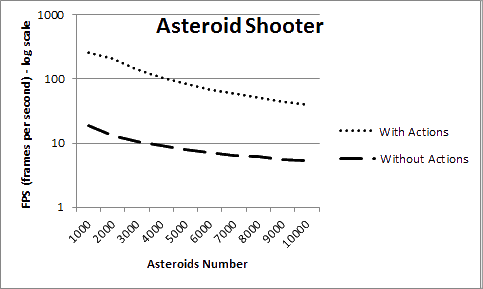
\includegraphics[scale=0.7]{Shooter.png}
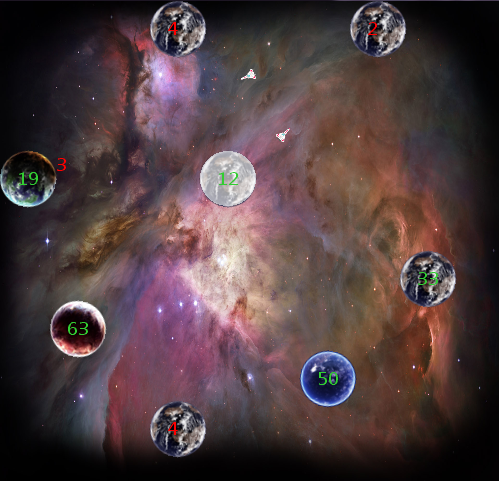
\includegraphics[scale=0.7]{RTS.png}
\caption{Frame rate as a function of numbers of entities.}
\label{fps_chart}
\end{figure} 

\section{Conclusions}
\label{sec:conclusions}
%% Changed by PS, April 4, 2014.

\section{Future work}
\label{sec:future_work}
The Casanova 2 language is capable of implementing usable and quite complex games. The language, while usable, is currently still in development as it misses a few features. In particular, support for multiplayer games is at this moment lacking. We believe that the existing mechanisms for handling time offered by Casanova 2 could be augmented with relatively little effort in order to greatly simplify the hard task of building multiplayer games. This is part of future work, that we are currently engaging in. We are also doing usability studies using students from various disciplines and backgrounds.

The high level view of the game that the Casanova 2 compiler provides can be exploited in order to improve the programmer experience. This means that we could use tools for code analysis (such as abstract interpretation \cite{nielson1999principles} or type system extensions) in order to better understand the game being built, and to help with correctness analysis, performance analysis, or even optimization.


%\subsection{User study}
%We wish to perform an in-depth user study for Casanova 2 to improve usability in the development process. We have already performed a partial (and quite promising) small user study which we will extend and complete.


%We have performed the following test: we gathered a group of students of game programming and a group of students of game design. We gave them a series of Casanova 2 samples, printed on paper. Each student had to guess the functionality of each sample, and sketch a screen-shot. Furthermore, each student also provided some additional feedback on the language.

%The samples were: (\textit{i}) a string of text moved around the screen with the keyboard, (\textit{ii}) a string of text that moves along a predefined path automatically, and (\textit{iii}) an asteroid shooter.

%Eleven (over a total of thirteen) students understood the samples completely, both drawing the screen-shots and explaining the dynamics of the game correctly. Two students were lost on the syntactic differences between Casanova 2 and the more familiar C-like syntax. The direct feedback was mostly centred around a series of common observations, which are reported in Table \ref{students_feedback}. For each observation, the table reports how many times we encountered it.

%\begin{table}[!t]
%% increase table row spacing, adjust to taste
%\renewcommand{\arraystretch}{1.3}
% if using array.sty, it might be a good idea to tweak the value of
% \extrarowheight as needed to properly center the text within the cells

%\caption{Feedback from students}
%\label{students_feedback}
%\centering

%% Some packages, such as MDW tools, offer better commands for making tables
%% than the plain LaTeX2e tabular which is used here.
%\begin{tabular}{|c||c|}
%\hline
%Syntax is unfamiliar at first & 3\\
%\hline
%Syntax is clear & 8\\
%\hline
%Indentation instead of parentheses is a downside & 2\\
%\hline
%List processing with queries is very effective & 1\\
%\hline
%Rules are a good abstraction for games & 2\\
%\hline
%\end{tabular}
%\end{table}

%We also built a significantly bigger sample, which we asked only three students to study. The sample is a checkpoint-based RTS (see Figure \ref{RTS game} for a screenshot). All students correctly identified the game mechanics, and provided some additional feedback. Most of this feedback overlaps with that obtained for the samples, but some new observations emerge. Arguably, some patterns become visible only with larger samples:
%\begin{itemize}
%\item \texttt{wait} and \texttt{when} are very powerful
%\item Multiple rules on the same field are very powerful
%\item Multiple rules on the same field may lead to behaviours that are complex to understand
%\end{itemize}


\section{Conclusions}
\label{sec:conclusions}

Casanova 2, a language specifically designed for building computer games, may offer a solution for the high development costs of games. The goal of Casanova 2 is to reduce the effort and complexities associated with building games. Casanova 2 manages the game world through entities and rules, and offers constructs (wait and yield) to deal with the run-time dynamics. As shown by the benchmarks in Section \ref{sec:evaluation}, we believe that we have taken a significant step towards reaching these goals. In fact, we achieved at the same time very good performance and simplicity, thereby empowering developers with limited resources. 

\end{document}
